\begin{pastexam}[label={px:ncku-109-comm-ds-03}]{成大電通所 109 學年度 第 3 題}
（問答）

Suppose we are given the preorder sequence\\
\hspace*{5em}A B C D E F G H I\\
and the inorder sequence\\
\hspace*{5em}B C A E D G H F I\\
of the same binary tree.\\
(a) Draw a binary tree defined by such a pair of sequences. (10 points)\\
(b) Does such a pair of sequences uniquely define a binary tree? (5 points)
\end{pastexam}

\begin{pastsoln}
\textbf{(a)} 前序的第一個是根，在中序裡找到根，左邊是左子樹、右邊是右子樹；左右子樹的前序就是根後面
接著的那兩段（長度和中序裡的兩段一樣），遞迴下去（資結書第~7.4~節）。
\begin{center}
\small
\begin{tabular}{llll}
\toprule
前序 & 中序 & 根 & 左子樹（中序） ／ 右子樹（中序） \\
\midrule
A B C D E F G H I & B C A E D G H F I & A & B C ／ E D G H F I \\
B C & B C & B & （空） ／ C \\
D E F G H I & E D G H F I & D & E ／ G H F I \\
F G H I & G H F I & F & G H ／ I \\
G H & G H & G & （空） ／ H \\
\bottomrule
\end{tabular}
\end{center}
$C$、$E$、$H$、$I$ 都只剩一個，是葉節點。 得到的樹：
\begin{center}
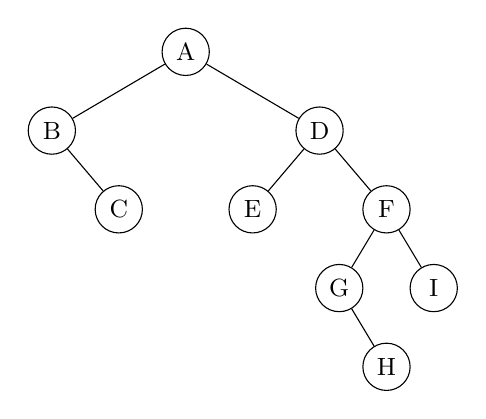
\begin{tikzpicture}[level distance=10mm,
  level 1/.style={sibling distance=34mm},level 2/.style={sibling distance=17mm},
  level 3/.style={sibling distance=12mm},
  every node/.style={circle,draw,inner sep=0pt,minimum size=6mm,font=\small}]
\node {A}
  child {node {B} child[missing] child {node {C}}}
  child {node {D} child {node {E}}
                  child {node {F} child {node {G} child[missing] child {node {H}}}
                                  child {node {I}}}};
\end{tikzpicture}
\end{center}
檢查：這棵樹的前序是 A B C D E F G H I，中序是 B C A E D G H F I，和題目一樣。

\textbf{(b)} 是，唯一（節點的名字都不同）。 理由就是 (a) 的做法每一步都沒有選擇（資結書定理~7.4）：
前序的第一個一定是根；中序裡根的位置唯一，決定了左子樹有哪些節點、幾個；前序裡根後面的那幾個就是
左子樹的前序，其餘是右子樹的前序。 對節點數歸納，左右子樹各自也被唯一決定，所以整棵樹唯一。

對照：只給前序和後序就不一定唯一，例如只有一個子節點時分不出它是左還是右（資結書定理~7.5）。 本題
B 只有右子節點 C、G 只有右子節點 H，換成前序加後序就分不出來了。
\end{pastsoln}
